% Section content template for individual Educative lessons
% This file contains the actual content for a specific section
% Generated from Educative API section content

% Section: Activity Diagram
% Section ID: 6705616068542464
% Section Slug: activity-diagram
% Generated: 2025-12-08T22:23:24.982225

An \textbf{activity diagram} is a communication diagram that is used to show the dynamic aspects performed by a system. This diagram is used to represent a series of actions, similar to how they may appear in a flowchart.

\subsection{Purpose of activity diagram}\label{-6BYVy7-YdaOkcRTcBX4M}
\\
Much like the previously discussed UML diagrams, activity diagrams are also used to show the sequence through which events occur in the system. Activity diagrams differ from other UML diagrams in that they specifically capture the message flow for each activity on to the next. These may look like flowcharts in appearance, but in execution, they can be much more. They can show various flows, such as single, parallel, concurrent, and branched.

\subsection{Components of an activity diagram}\label{BNFVMMnDg8nAB1V2KieT3}
\\
Various components make up an activity diagram. Let\textquotesingle s discuss some of the essential features of this diagram that appear most often.
\\
\textbf{Initial:} This represents the start of the workflow of the activity diagram. They can be visualized as the node in a tree structure.

\begin{figure}[htbp]
 \centering
 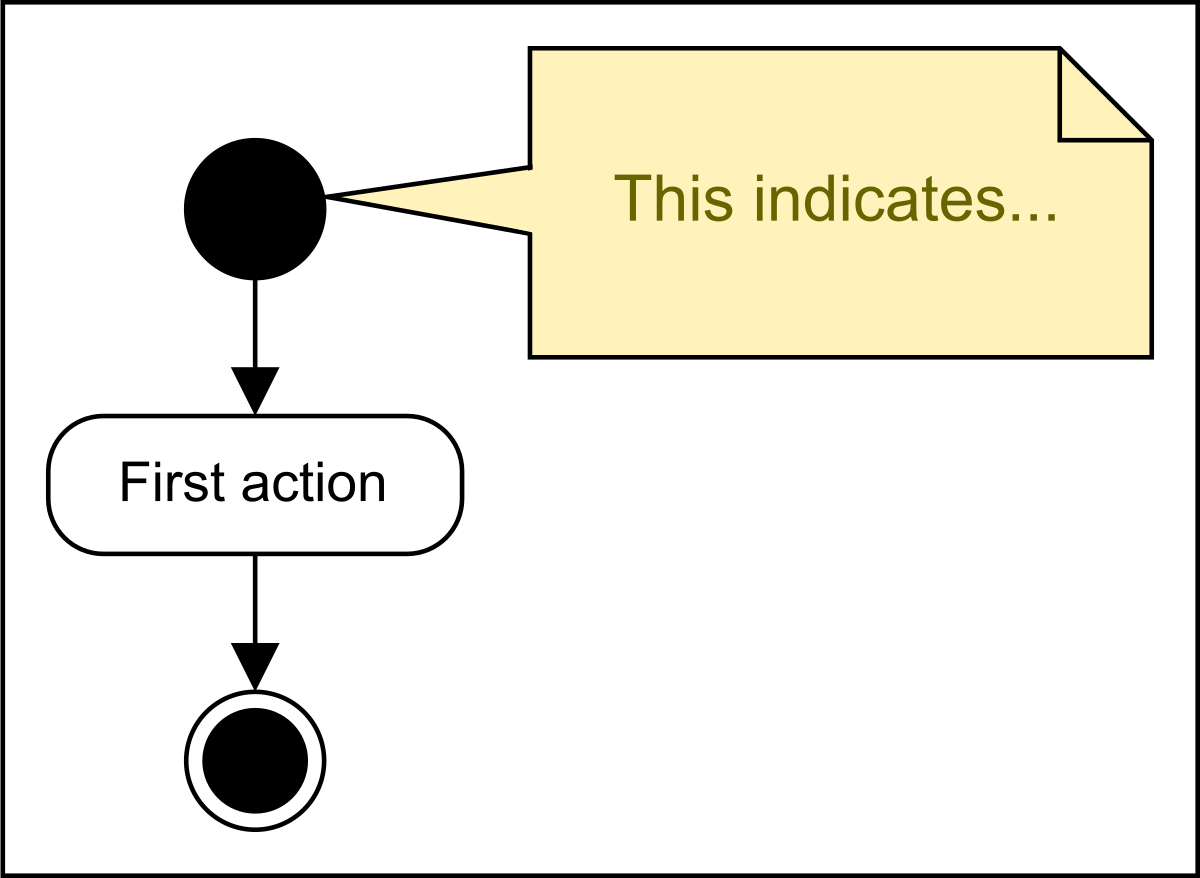
\includegraphics[width=0.25\textwidth]{Images/chapter_3/section_6705616068542464/5722301905764352.png}
 \caption{Initial node in an activity diagram}
\end{figure}

\textbf{Action:} These are the main building blocks of an activity diagram and are used to show the activities that a modeled process is made of.

\begin{figure}[htbp]
 \centering
 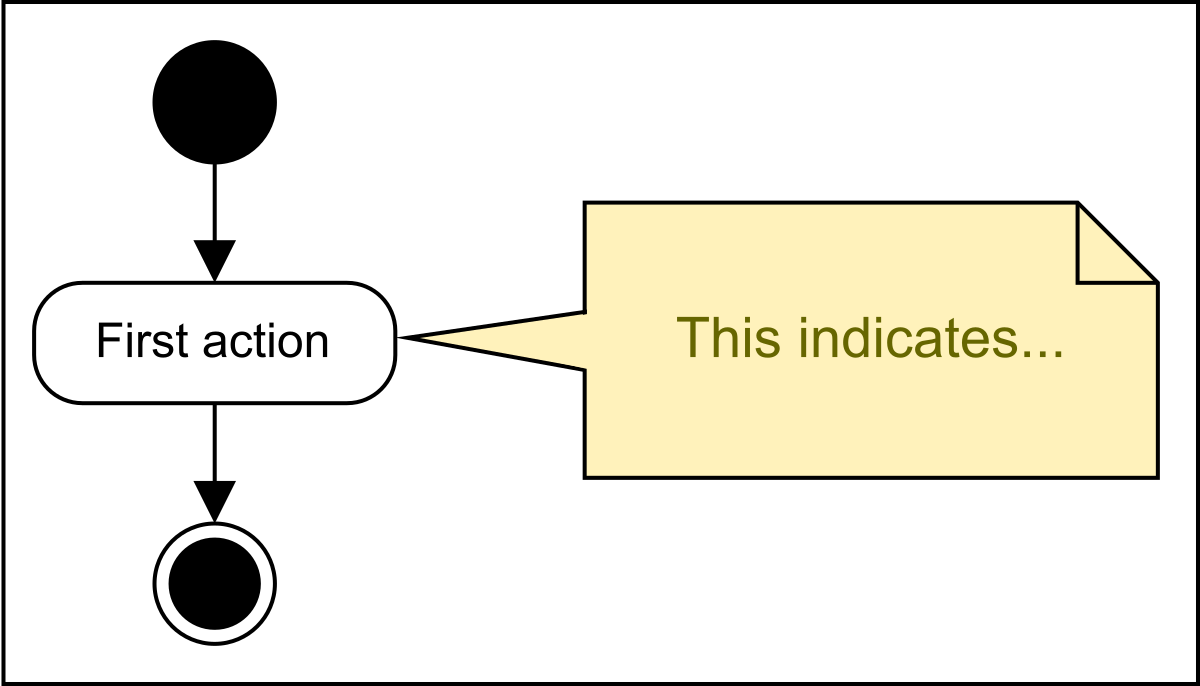
\includegraphics[width=0.25\textwidth]{Images/chapter_3/section_6705616068542464/4516638768758784.png}
 \caption{Action in an activity diagram}
\end{figure}

\textbf{Flow final:} This represents the end of a single path in the activity diagram. They can be visualized as a leaf in a tree structure.

\begin{figure}[htbp]
 \centering
 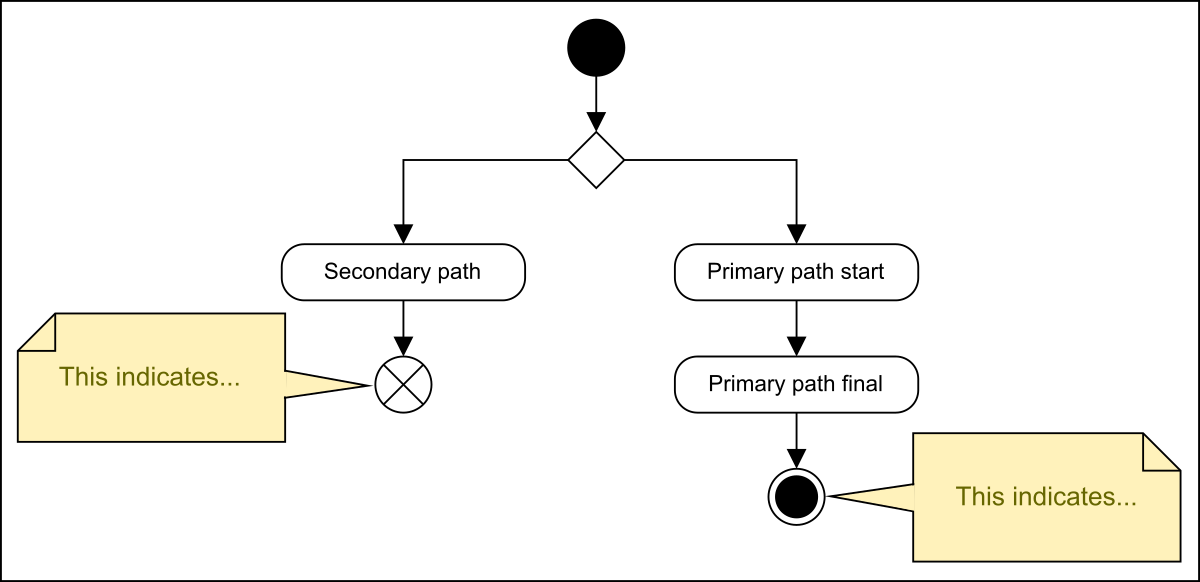
\includegraphics[width=0.25\textwidth]{Images/chapter_3/section_6705616068542464/5973660613869568.png}
 \caption{Flow final in an activity diagram}
\end{figure}

\textbf{Activity final:} This represents the end of all the activities in the activity diagram.

\begin{figure}[htbp]
 \centering
 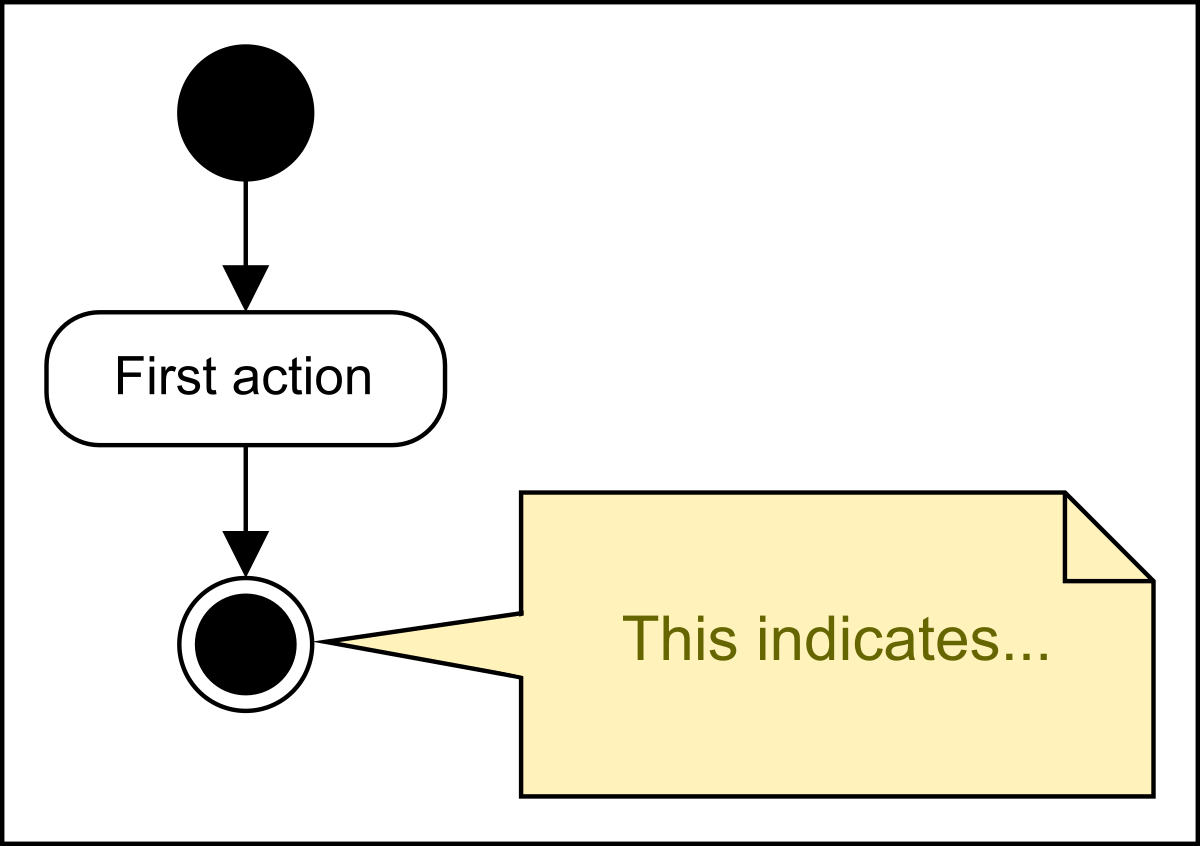
\includegraphics[width=0.25\textwidth]{Images/chapter_3/section_6705616068542464/6407315534381056.png}
 \caption{Activity final an activity diagram}
\end{figure}

\textbf{Control flow:} This shows the directional flow of the diagram. This exists as a connector between one action and another.

\begin{figure}[htbp]
 \centering
 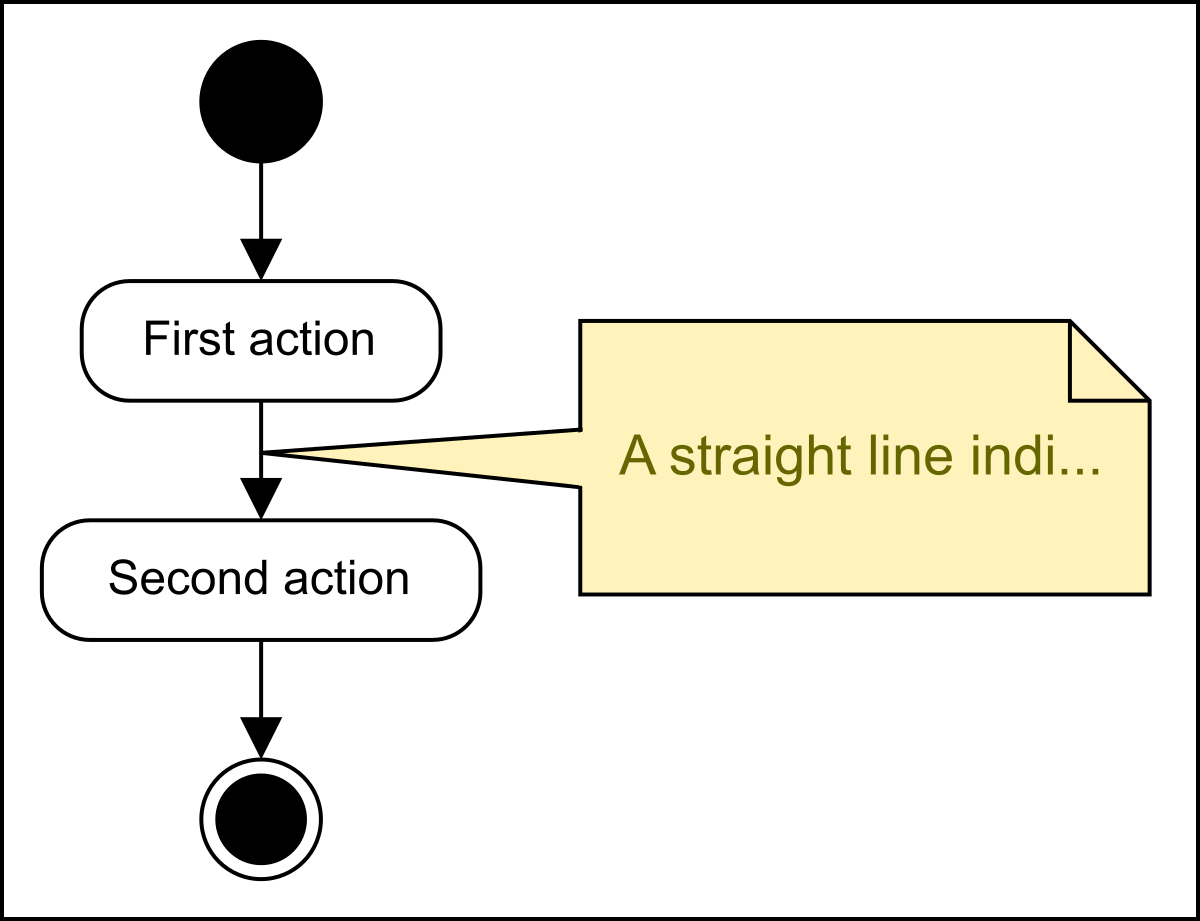
\includegraphics[width=0.25\textwidth]{Images/chapter_3/section_6705616068542464/6168354928984064.png}
 \caption{Control flow in an activity diagram}
\end{figure}

\textbf{Object flow:} This shows the path of the objects as they move throughout the activity.

\begin{figure}[htbp]
 \centering
 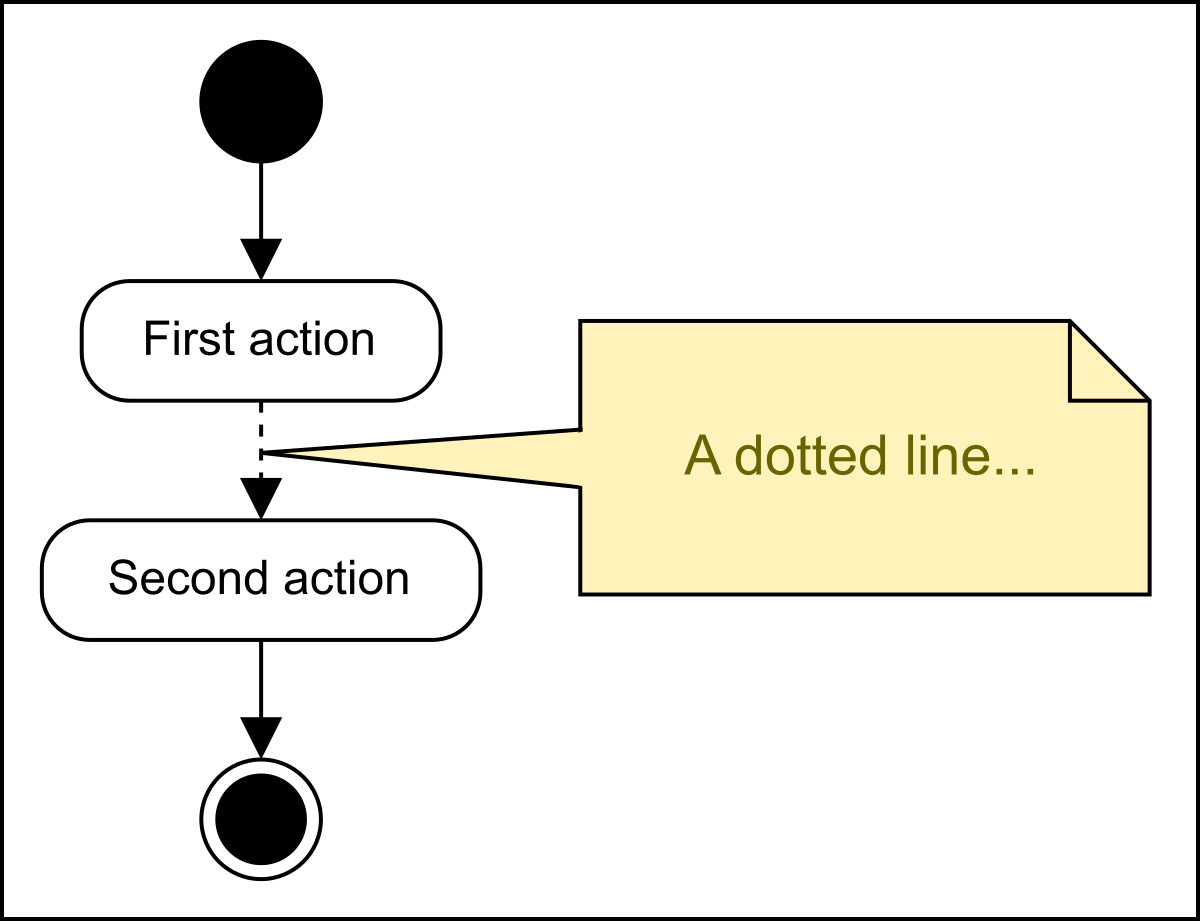
\includegraphics[width=0.25\textwidth]{Images/chapter_3/section_6705616068542464/5332627184418816.png}
 \caption{Object flow in an activity diagram}
\end{figure}

\textbf{Decision:} This is used to represent multiple options that are possible in a system. They appear as a branch alongside the text describing the condition for the path.

\begin{figure}[htbp]
 \centering
 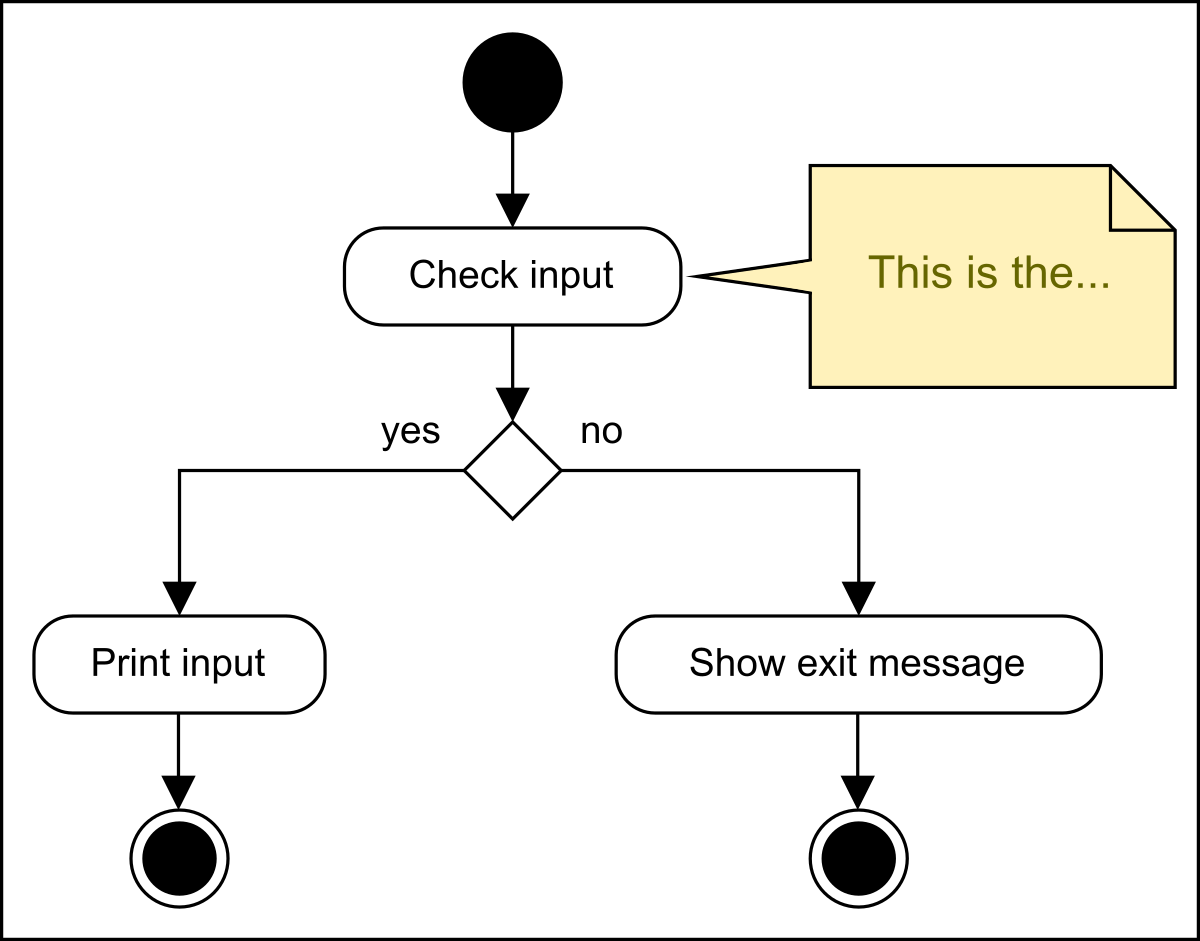
\includegraphics[width=0.25\textwidth]{Images/chapter_3/section_6705616068542464/5683150711947264.png}
 \caption{Flow final in an activity diagram}
\end{figure}

\textbf{Merge:} This uses the same symbol as a decision. However, this shows that multiple options join at this node, but leads to a single output.

\begin{figure}[htbp]
 \centering
 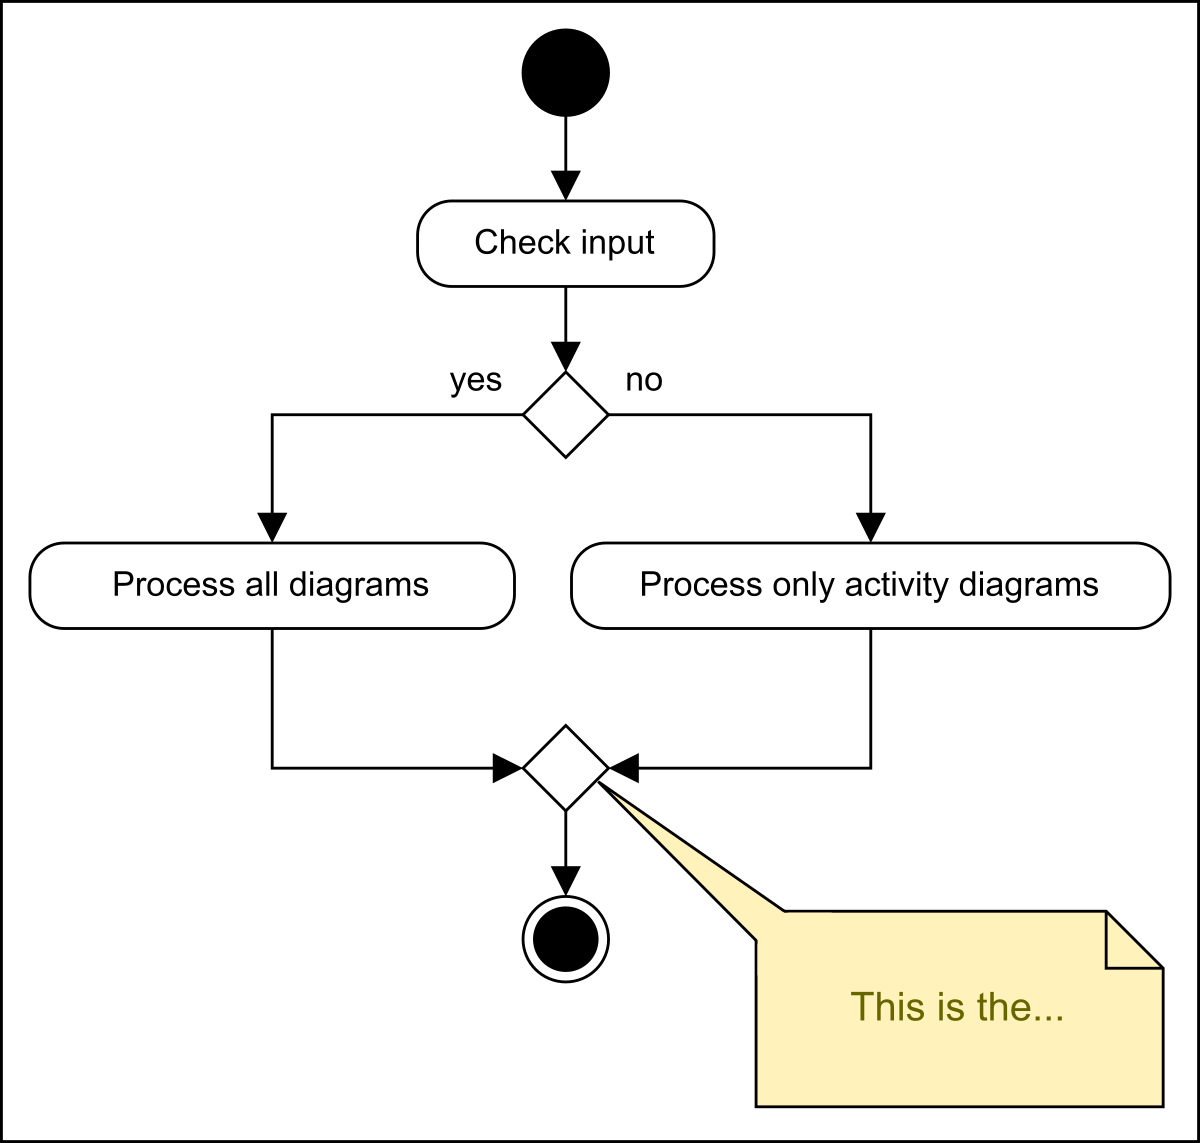
\includegraphics[width=0.25\textwidth]{Images/chapter_3/section_6705616068542464/6006189932675072.png}
 \caption{Flow final in an activity diagram}
\end{figure}

\textbf{Fork and join:} The fork node represents a single activity that is split into two concurrent activities happening alongside each other. On the other hand, the join node joins two concurrent activities together to lead to a single activity.

\begin{figure}[htbp]
 \centering
 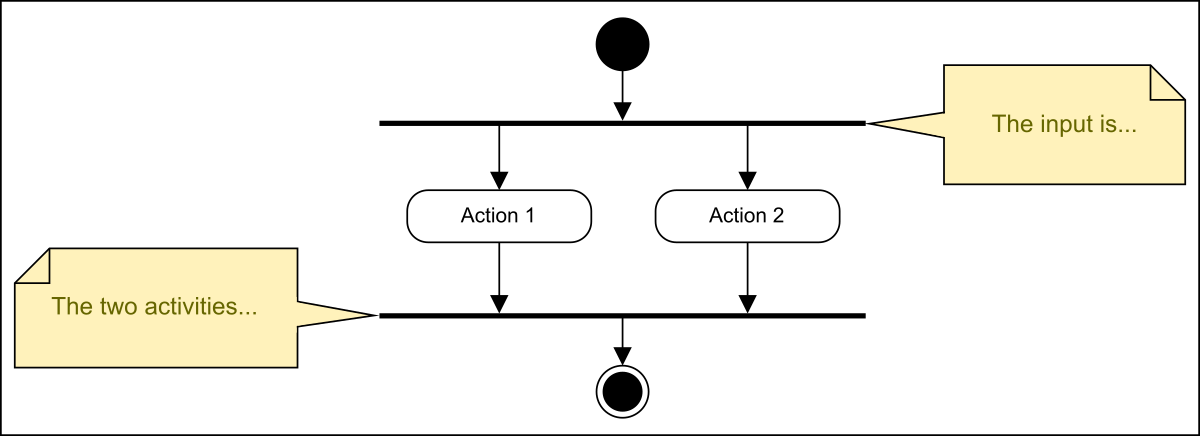
\includegraphics[width=0.25\textwidth]{Images/chapter_3/section_6705616068542464/4541895458160640.png}
 \caption{Fork and join in an activity diagram}
\end{figure}

\subsection{How to draw an activity diagram}\label{43mxzQ9MuFA09eMB7Iu8q-9}
\\
Activity diagrams show the message flow of actions in a simple manner. Before we start, it is important to understand that there isn\textquotesingle t one correct way of creating an activity diagram. Some of us may have a different approach to handling these problems.
\\
This lesson introduces a methodology that helps break down the problem into smaller, achievable tasks.

\subsubsection{Determine the actions of the system}\label{NwK4TwqI8ZTHq5z4rGF-C}
\\
Here we need to recognize each action and how they interact with the others in the system. We can use the aid of use cases to make this process easier.
\\
For now, we will use the previous example where a customer wants to withdraw cash from an ATM.

\begin{figure}[htbp]
 \centering
 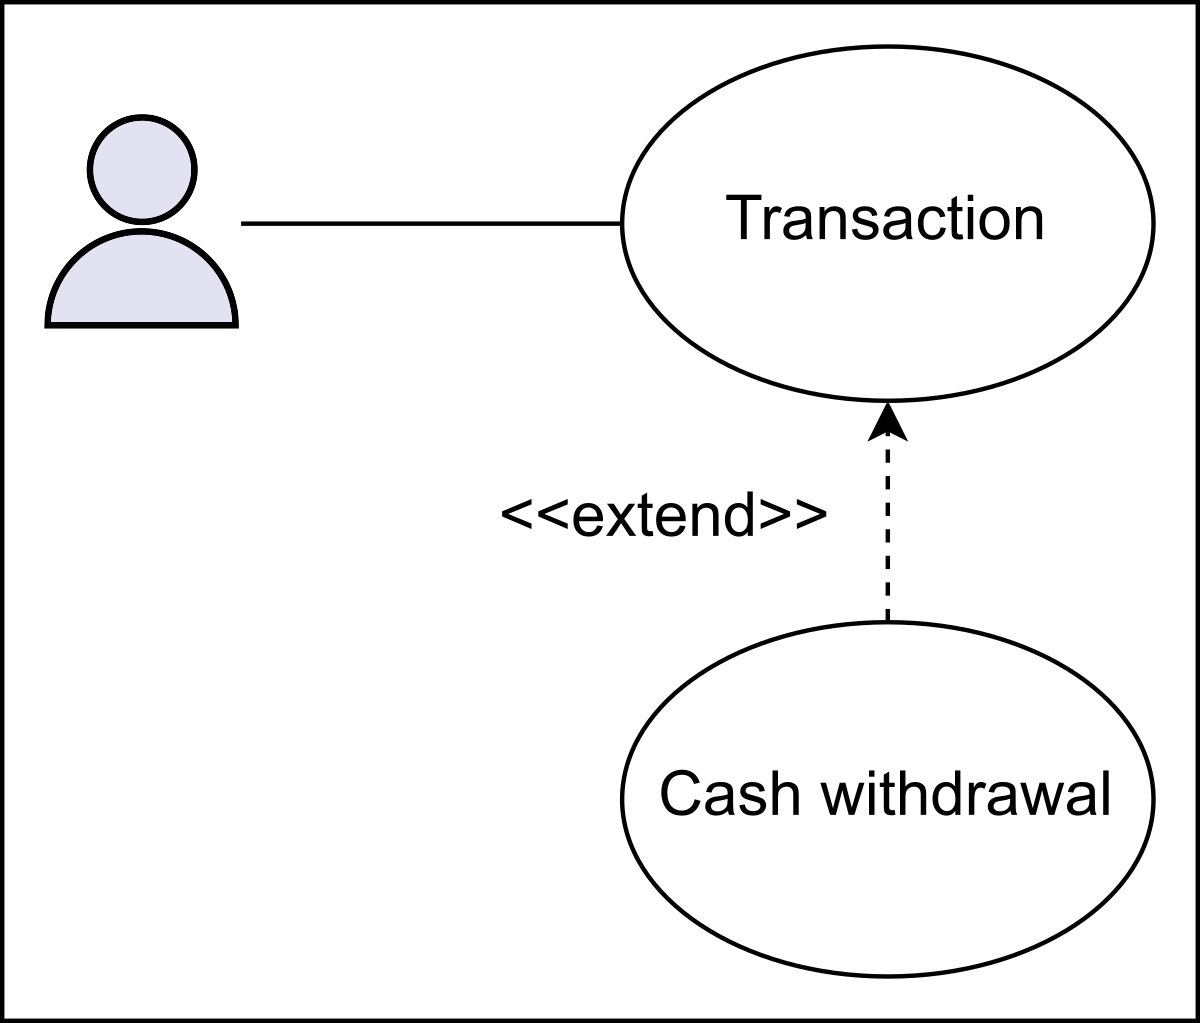
\includegraphics[width=0.25\textwidth]{Images/chapter_3/section_6705616068542464/5462020545839104.png}
 \caption{Use case for cash withdrawal}
\end{figure}

Determine the actors and their roles, and list down all the actors and objects that will be involved in the entire message flow of the activity. These would be the following:

\begin{itemize}
\item
\protect\phantomsection\label{jFvdwOQSQJ4jsRl_UuqKV}
Customer
\item
\protect\phantomsection\label{vmZrQglcK6h-CmSdMfDHb}
ATM
\item
\protect\phantomsection\label{edR_aY3uuBGWijwnvvd1V}
Transaction
\item
\protect\phantomsection\label{oPBfCKWXuT11_ZqDXJNQx}
Account
\item
\protect\phantomsection\label{mOQA4CbfVmWqsA6_CahKo}
Cash dispenser
\end{itemize}

\subsubsection{Finding the flow of each activity}\label{taJ09Q1hwrneiEav66PhE}
\\
We first work out the order in which the actions should occur, and we also note down the action that coincides with the other actions. Here , we also determine the conditions that lead to specific outcomes. Lastly
, we note if there are actions that can only be executed once a previous one is completed.

\subsubsection{Create the diagram}\label{Txo9Rnpp5s-QPdDO1e8Xf}
\\
Now, we will use these steps to build a sample activity diagram.

\begin{figure}[htbp]
 \centering
 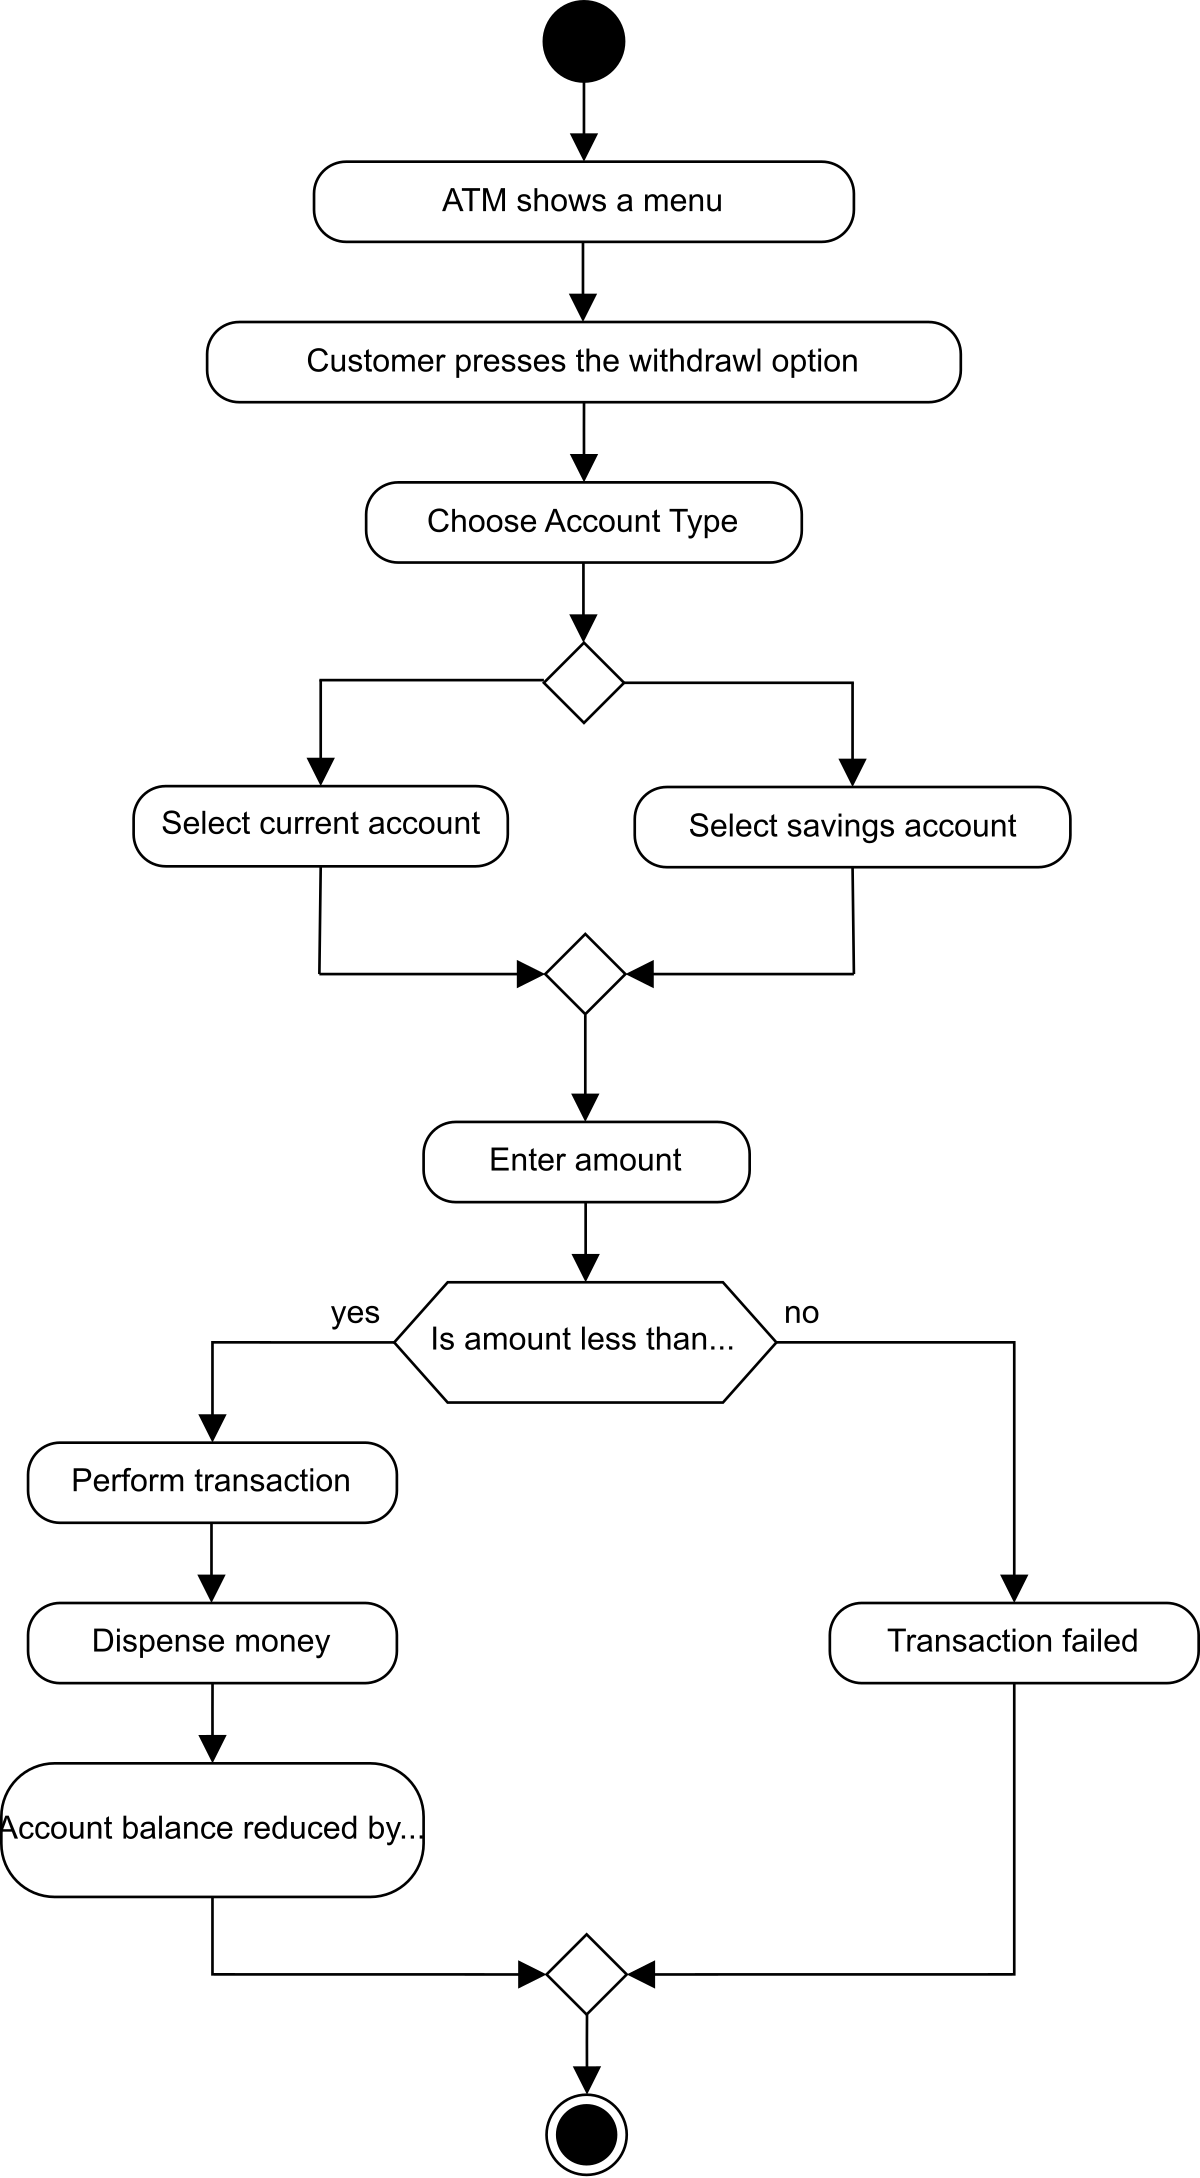
\includegraphics[width=0.5\textwidth]{Images/chapter_3/section_6705616068542464/5146812176138240.png}
 \caption{An example of a cash withdrawal from an ATM}
\end{figure}

\subsection{Sequence vs. activity diagram}\label{gXirk4Wsa8-vPaxPQM1US-2}
\\
We have now studied both the sequence and the activity diagram. As a refresher, the following table provides an overview of the differences that exist between both of them:

\begin{table}[htbp]
\centering
\small
\adjustbox{max width=\textwidth}{
\begin{tabular}{|p{0.486\textwidth}|p{0.464\textwidth}|}
\hline
\textbf{Sequence Diagram} & \textbf{Activity Diagram} \\
\hline
\hline
It is used for dynamic modeling. & It is used for functional modeling. \\
\hline
It visualizes the flow of messages from one object to the other. & It visualizes the flow of messages from one activity to the other. \\
\hline
It helps in modeling the systems workflow. & It helps in visualizing a systems sequence of calls for a particular functionality. \\
\hline
It describes the behavior of various objects just for an independent use case. & It describes the general sequence of actions for various objects as well as various use cases. \\
\hline
\end{tabular}
}
\end{table}

Now that we have learned the conventions and benefits of these types of UML diagrams, let\textquotesingle s test these concepts in the next lesson.

% End of section content